\documentclass[a4paper,12pt]{article}
\usepackage{color}
\usepackage{graphicx}
\usepackage{listings}

\usepackage{hyperref}

\usepackage{float}

\begin{document}

\title{Bhargava Design Handbook}
\author{Aman Bhargava}
\date{\today}
\maketitle

\tableofcontents

\section{Identity}
\subsection{A Brief Biography}
My name is Aman Bhargava, and I am currently an Engineering Science student at the University of Toronto. I was born and raised in the state of Maine in the United States, and I moved to Cobourg, Ontario when I was 12.

\subsection{My Values}
I value altruism, creativity/open-mindedness, efficiency, and practicality. Figure 1 represents the flowchart of goodness I see these forming.

\begin{figure}[H]
\centering
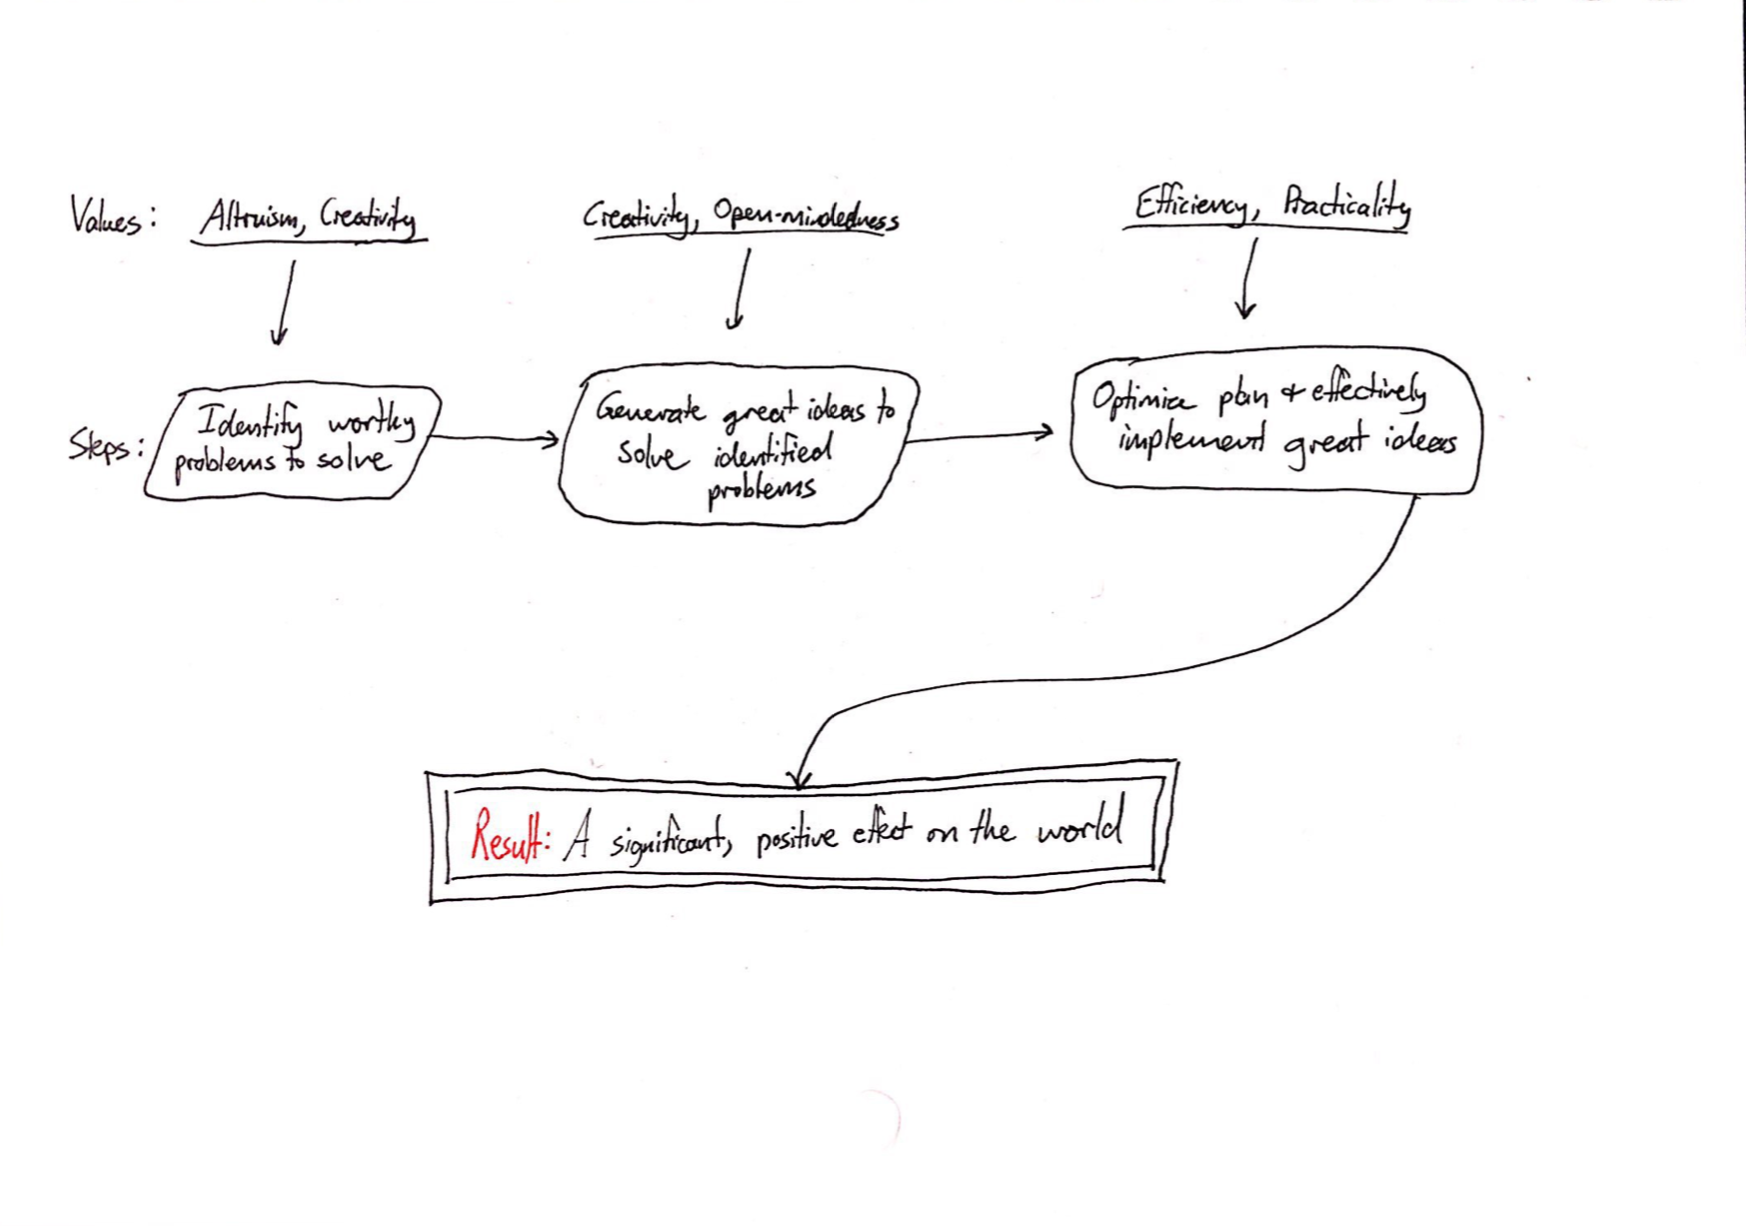
\includegraphics[width=0.9\textwidth]{img/image001.png}
\caption{How my values integrate with the steps to my goal of significantly and positively changing the world.}
\label{}
\end{figure}

I believe that this general cycle has the power to have a significant and positive effect on the world, which is one of my most deeply-held ambitions in life.

\subsection{Skills}
\begin{enumerate}
\item Team organization and leadership: Through my experience in leading group projects in school, university, hackathons and more, I have learned how to run an effective, goal-driven team.
\item Programming: I have confidence in my ability to implement ideas into software, at least in such a way that can communicate a basic idea.
\item Data Analysis: I am competent with data visualization, basic statistics, supervised machine learning, and basic clustering.
\item Fabrication: I am competent with basic fabrication tools, namely those found in the Light Fabrication Facility (3D-printing, laser cutting, foam core, basic carpentry, arduino/raspberry pi programming)
\item Argumentation: As a former provincial debater, I believe in my ability to effectively use argumentation to get closer to the truth in the vast majority of issues that I am able to understand.
\item Research: I am able to effectively utilize engineering and scholarly libraries and databases to get the information that I need.
\item Self-learning: My ability to learn things as needed on my own has proven useful time and time again in all of my projects.
\end{enumerate}

\subsection{Biases}
Everything I have written so far in this introduction is a potential bias. Due to my experience in programming, I am likely overly willing to go down the technological route to solve problems without considering non-technological solutions. Because I pride myself in my ability to teach myself, I am less likely than would be optimal to ask for help or consider the possibility of a project being out of my abilities.

Beyond the biases I have implicitly defined in this introduction, I think that my personality makes me overly willing to go outside the box for projects. Because I value creativity so highly, I find it boring to go by the book and am susceptible to the temptation of going outside the box even when it might not be favourable for the design objective.

More generally, I am biased by what I think is “boring” and “interesting”. Even when I try not to, one of the first things I think of when I consider a design alternative or process idea is how “cool” it seems. Even if an alternative will meet the needs of our requirements model/our stakeholders’ needs, I will be turned off of it if it doesn’t meet my subjective, unconscious criteria for what is “interesting”.

Finally, I have been in private schools for my entire life. Simultaneously, I have frequently visited my parent’s home country of India, where I have been exposed (for several weeks at a time) to extreme poverty. I have most of my time around two ends of the socio-economic spectrum, and I am almost certainly biased by that extremism, though I find it difficult to predict exactly how.

\subsection{Metadiscourse on Handbook Design}
I will go on to discuss my projects, including the process followed and holistic review for each, followed by a description and justification of my personal design process, and finally a full overview of all the tools, models, and frameworks mentioned and briefly discussed in the projects section.

My handbook is organized this way because my projects are a core part of my identity and therefore ought to be introduced first to better understand my use of tools and the derivation of my personal design process. I choose to be detailed about my projects because, in my experience in writing guides for my future self, I require many mental hooks to draw upon in order to recall concepts, ideas, and skills optimally.

This organization also mirrors my value system organization. I introduce my projects (i.e. ‘identifying worthy problems to solve’), then my personal design process (i.e. a tool to ‘generate creative, good solutions to these problems’), and finally close with detailed description of each engineering design tool (i.e. methods to ‘optimize my plan and effectively implement the great ideas’).

I chose not to group my Tools into categories such as FDCR because I invented many of them and many are from outside of Praxis lectures, so they don’t fit directly into easily describable categories. As well, when I am looking through in the future, being forced to look through all my favourite tools will help me to potentially creatively alter a tool that wouldn’t initially fit the use case, but could both my project via its effectiveness and actualize my values of creativity and open mindedness.

My invented tools are valid because I have evidence in the form of my experience that they work for me. Since this handbook is meant for my future design work, I am a key stakeholder and that it plenty of reason to be valid. On top of this, I incorporate further research to justify why many of my invented tools are valid.




\section{Projects}
\subsection{Importance of Projects}
I have always been a project-oriented person, and I love doing projects. Using projects as case studies has been extremely valuable for my success in later projects. The following is a brief summation of some of my projects from the past year, since the beginning of Praxis I. I will present them in chronological order, discussing the project goals, process, and a brief holistic review.

\subsection{Praxis I Design - Smart Hat}
For our Praxis I design project, Alice, Kelvin and I worked to improve the quality of sleep for Engsci’s in transit. We designed for effectiveness in terms of light and sound blockage, along with cost, comfort, durability, and aesthetics.

\subsubsection{Process}
We diverged a multitude of ideas using tools such as \textbf{extreme DfX} and then converged to a conceptual design via \textbf{system 1.5 analysis} and comparing our alternatives using high-level objectives via \textbf{logical argumentation and research}. We built a low-fidelity prototype using a Santa hat and a pair of cheap headphones to demonstrate our idea and to get a sense of the scale. Then, we used the \textbf{divide and conquer} design tool to divide our design exercise into many smaller design problems and did smaller rounds of framing, diverging, and converging for each detailed design decision. This enabled us to turn our conceptual design into a detailed, well-substantiated design.

\begin{figure}[H]
\centering
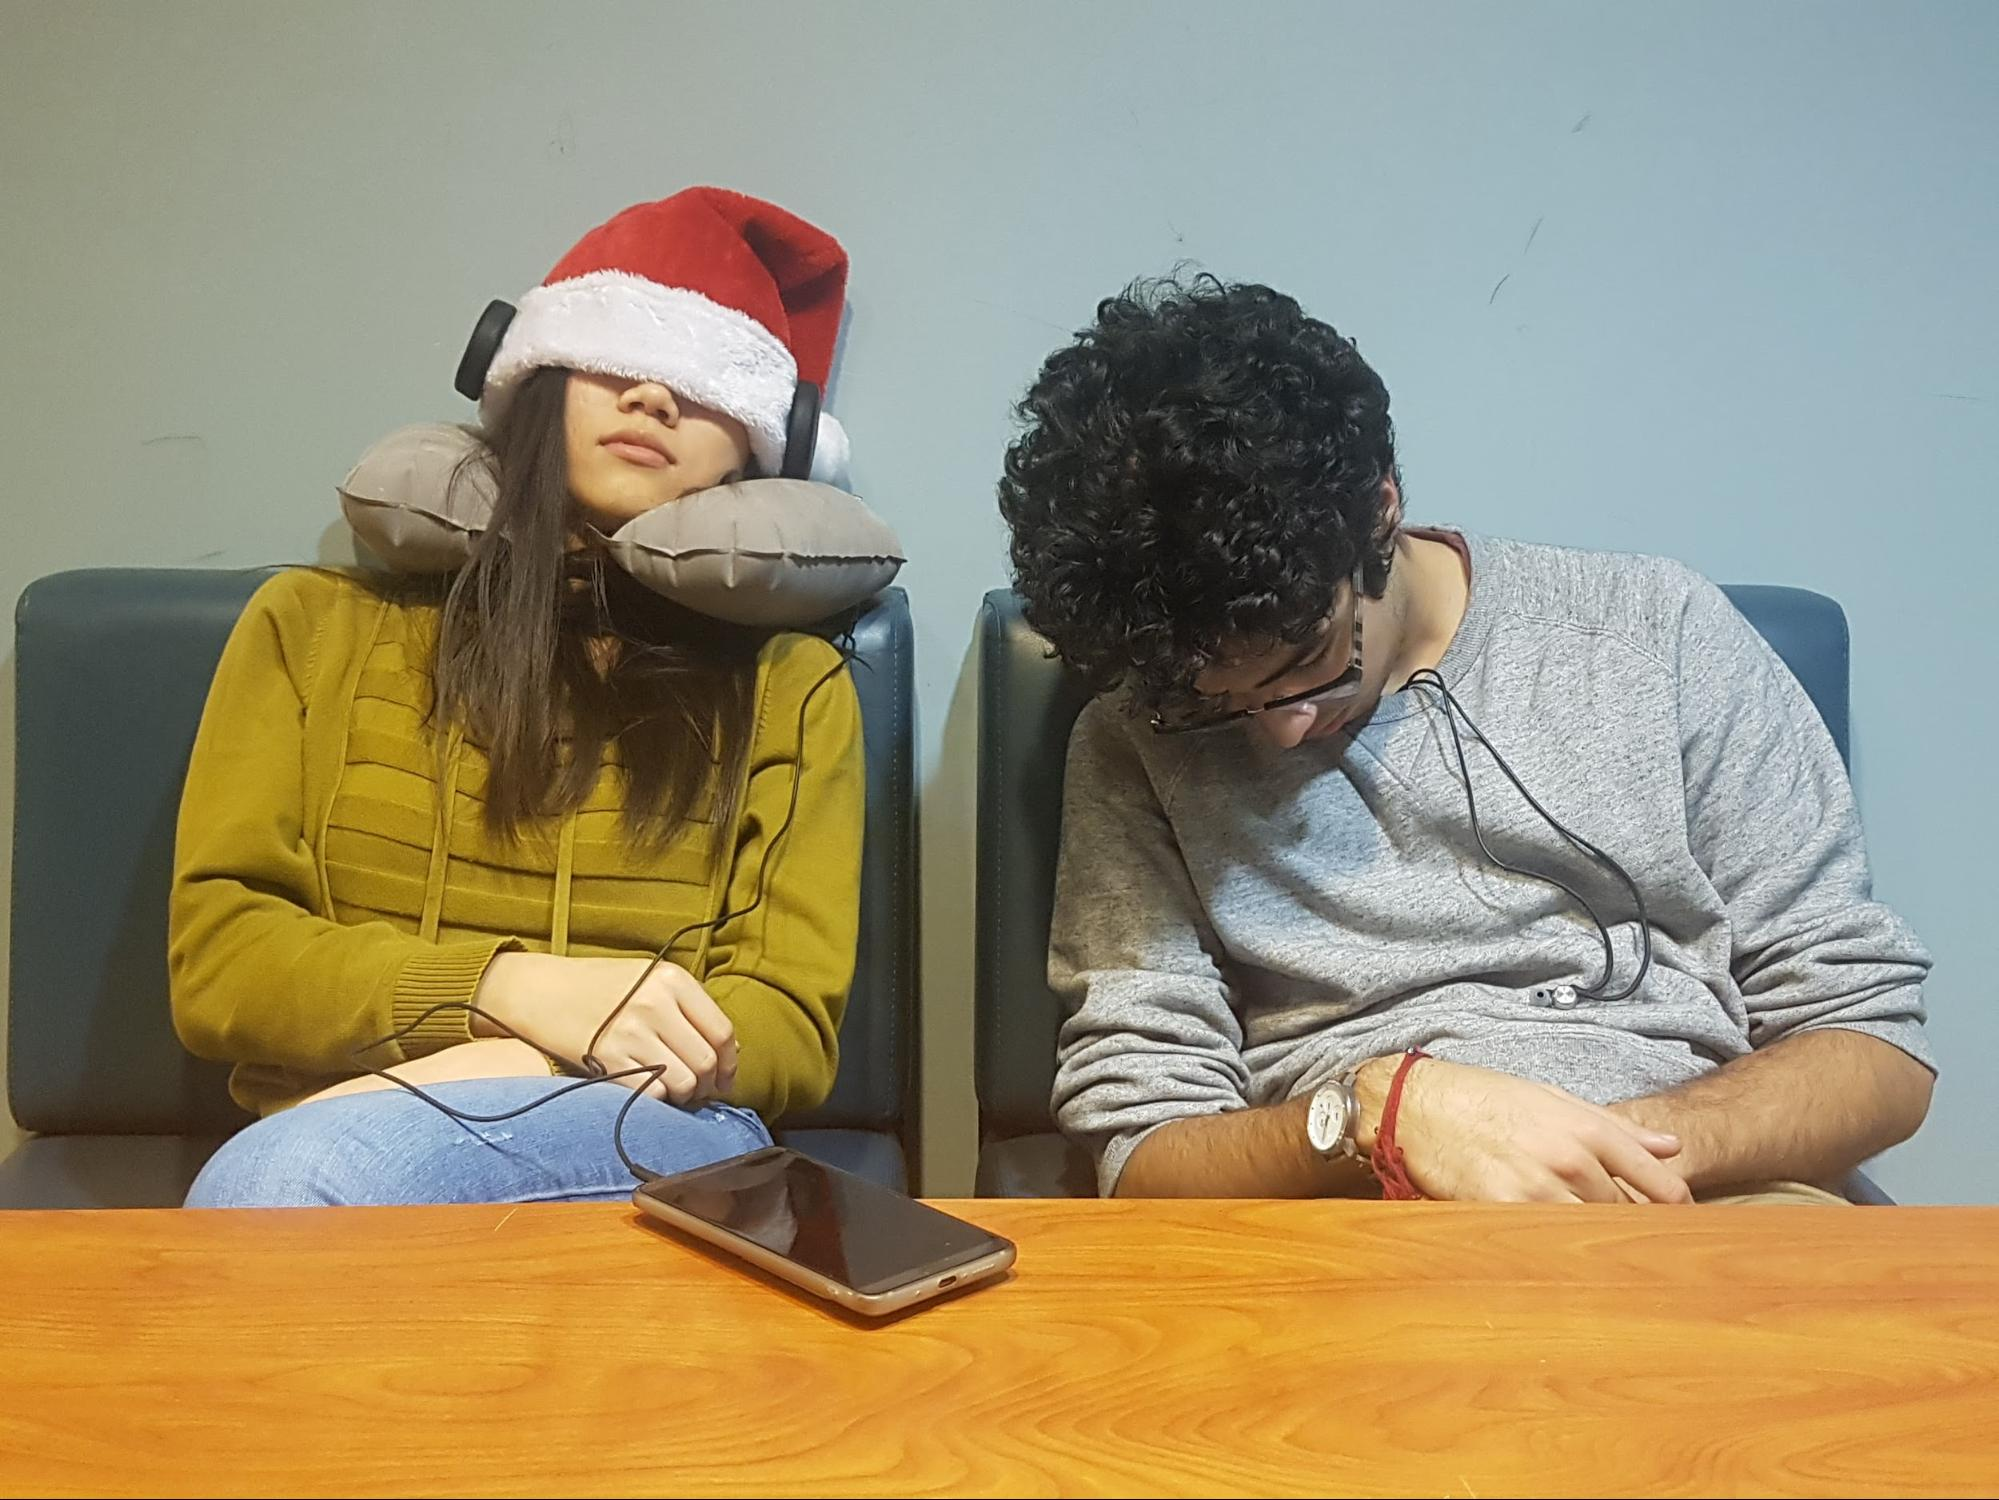
\includegraphics[width=1\textwidth]{img/image002.jpg}
\caption{Demonstrating beta prototype. Our final design retained the shape presented but used \textbf{divide and conoquer} to add rigour to the fine details.}
\label{}
\end{figure}

\begin{figure}[H]
\centering
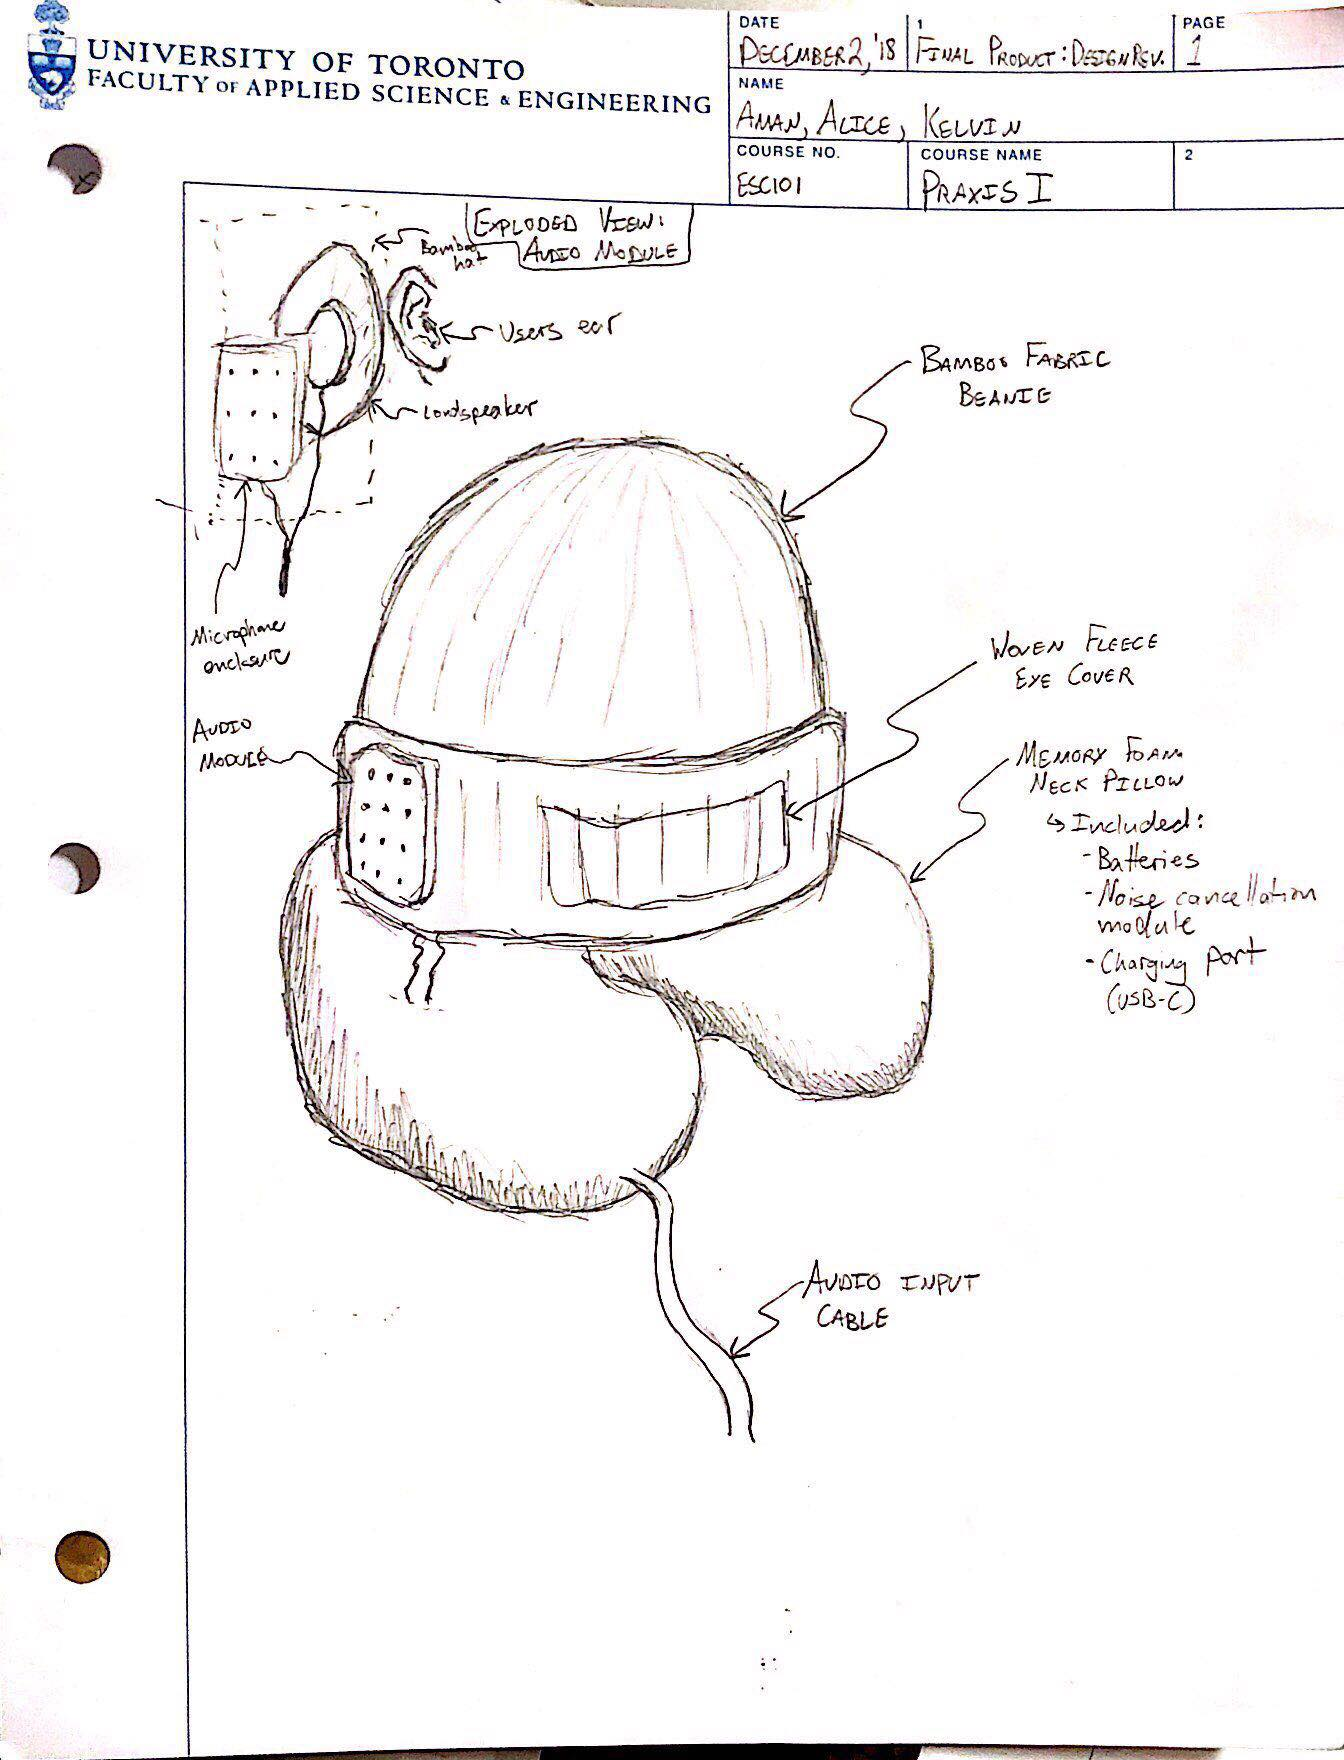
\includegraphics[width=1\textwidth]{img/image003.jpg}
\caption{Our final design, post divide and conquer. The design is far more specific and rigorous than the beta version, but is remains informed by the initial design.}
\label{}
\end{figure}

\subsubsection{Holistic Review}
Overall, I believe that we made a well-argued case for our design. We had comprehensive research and strong prototyping, but I believe that we were rather held back by our attachment to dogmatic design. We were concerned more about the quality of our grades rather than the quality of our designs. Because of this, we were overly attached to the design process discussed in class. We initially did not realize that we were allowed to break our design decision into multiple smaller design decisions. Because of this, we thought that we would need to go through a tremendous number of fully-fledged alternatives in order to arrive at a ‘well justified’ final design. It was only after I drafted this alternative journey 3 days before the due date that we were able to really move forward well.

The biggest lesson learned was that the design process is malleable. If one can come up with a good reason to change the design process to better fit the opportunity at hand, it is their duty as an engineer to at least argue for that change in the design process.

\begin{figure}[H]
\centering
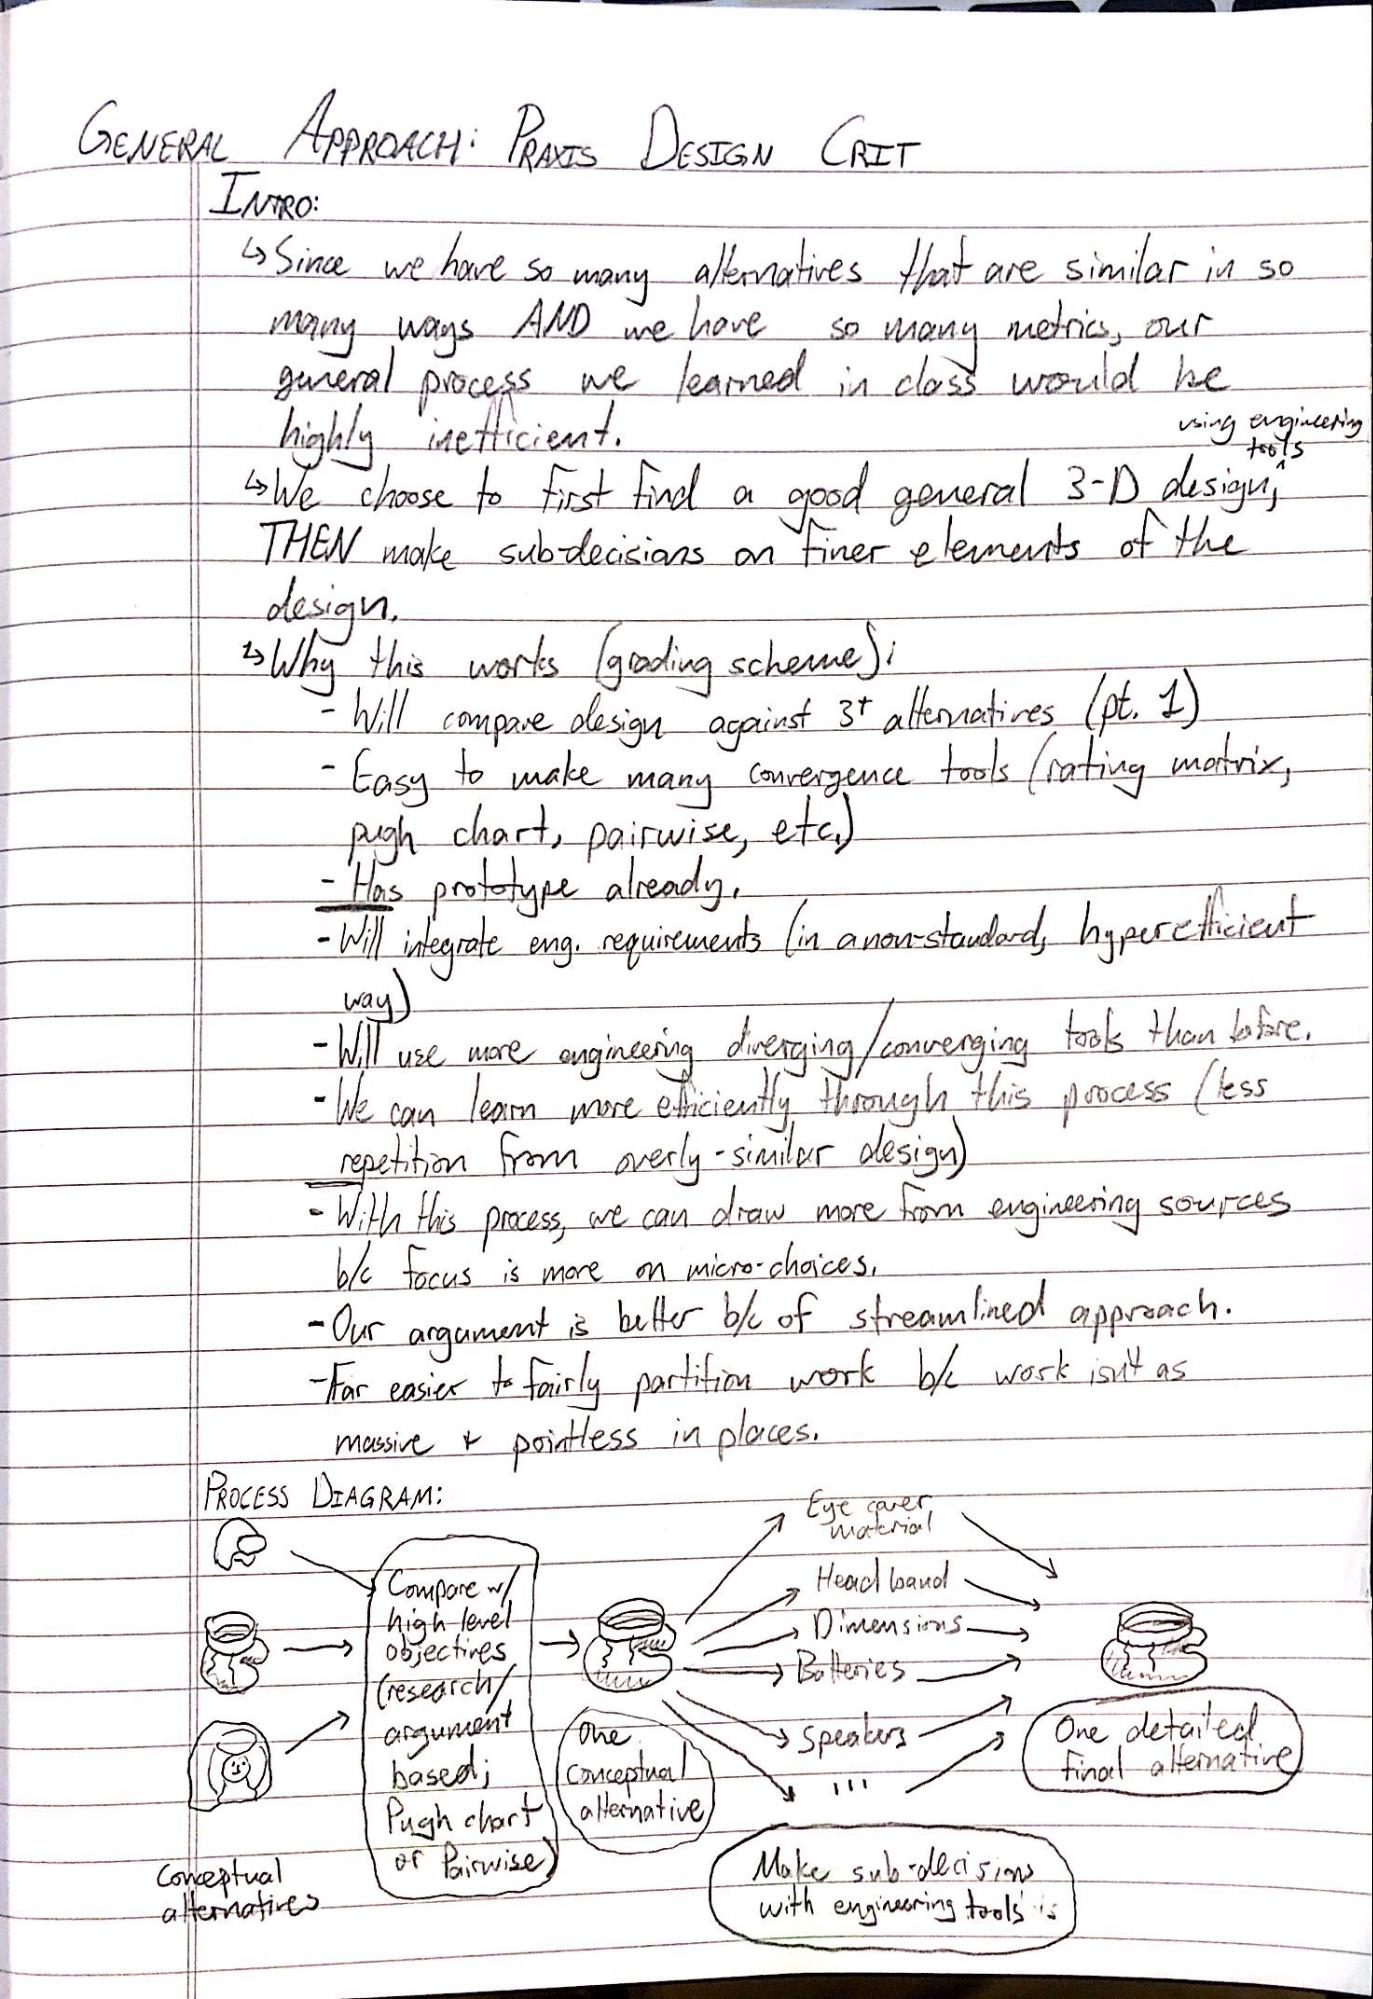
\includegraphics[width=1\textwidth]{img/image004.jpg}
\caption{My initial proposal for the group to use the 'divide and conquer' method to finalize our design. The experience of changing the design process influenced the rest of my projects and my personal design process profoundly.}
\label{}
\end{figure}


\subsection{CIV102 - Genetic Bridge Algorithm}
The CIV102 bridge project is a staple of Engsci, but my biggest takeaway from it was a ‘side project’ of sorts that stemmed from the main project. We were tasked with making a matboard bridge that could hold the maximum amount of weight under some specified loading conditions. In class, we learned the formulae that would give the amount of weight a bridge would hold before failing by some arbitrary failure mechanism.

\subsubsection{Process}

As soon as I saw this assignment, I saw how it could easily be made into an optimization problem; the project had clear objective functions (formulae for failure loading), constraints (amount of matboard) and structure (a bridge). After discussing with our team, we decided it would be in our best interest if I were to take the time to code our bridge measurement formulae and attempt to make an optimization algorithm to generate the parameters for our bridge design. We came to this decision via an \textbf{expected value calculation} - we looked at the potential benefit to our grade (25\% bonus for ‘creative solutions’) and my chances of success (estimated fairly high given my background in programming and genetic algorithms).

I chose a genetic algorithm because it mirrors the design process that Professor Collins teaches - it is literally a \textbf{rapid, (automated) iterative design process}. This worked fantastically well in creating extremely strong bridge designs (designs predicted to withstand more than 3 kilonewtons), and our group was still able to do well despite the fact we struggled with implementing the design due to the fact that we managed the risk well (performed \textbf{expected value calculations}).

\begin{figure}[H]
\centering
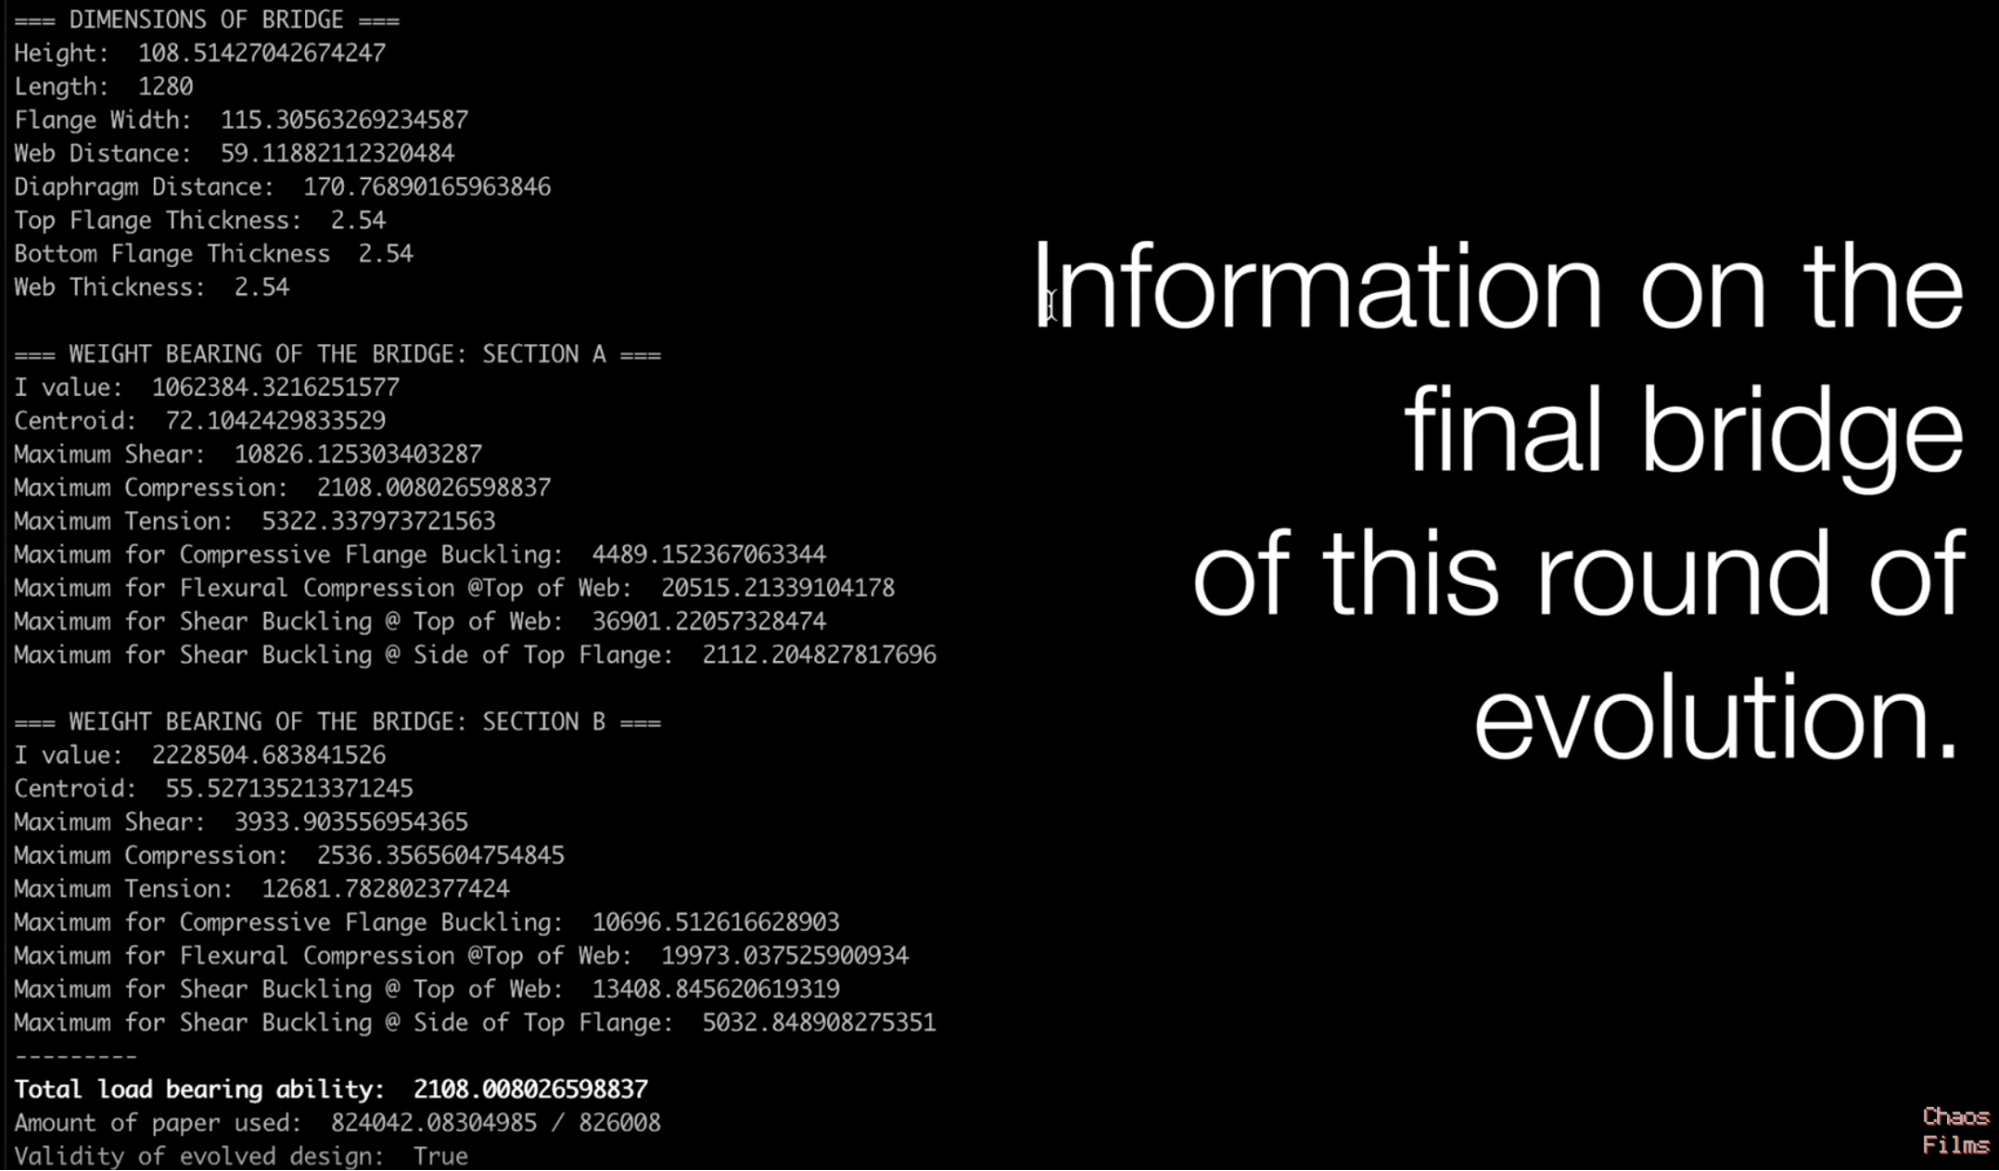
\includegraphics[width=0.7\textwidth]{img/image005.png}
\caption{The output of the evolution program. This improved our \textbf{expected value calculations} because we could test it against our paper calculations easily and trace bugs in the code back to their functions based on this output.}
\label{}
\end{figure}

\begin{figure}[H]
\centering
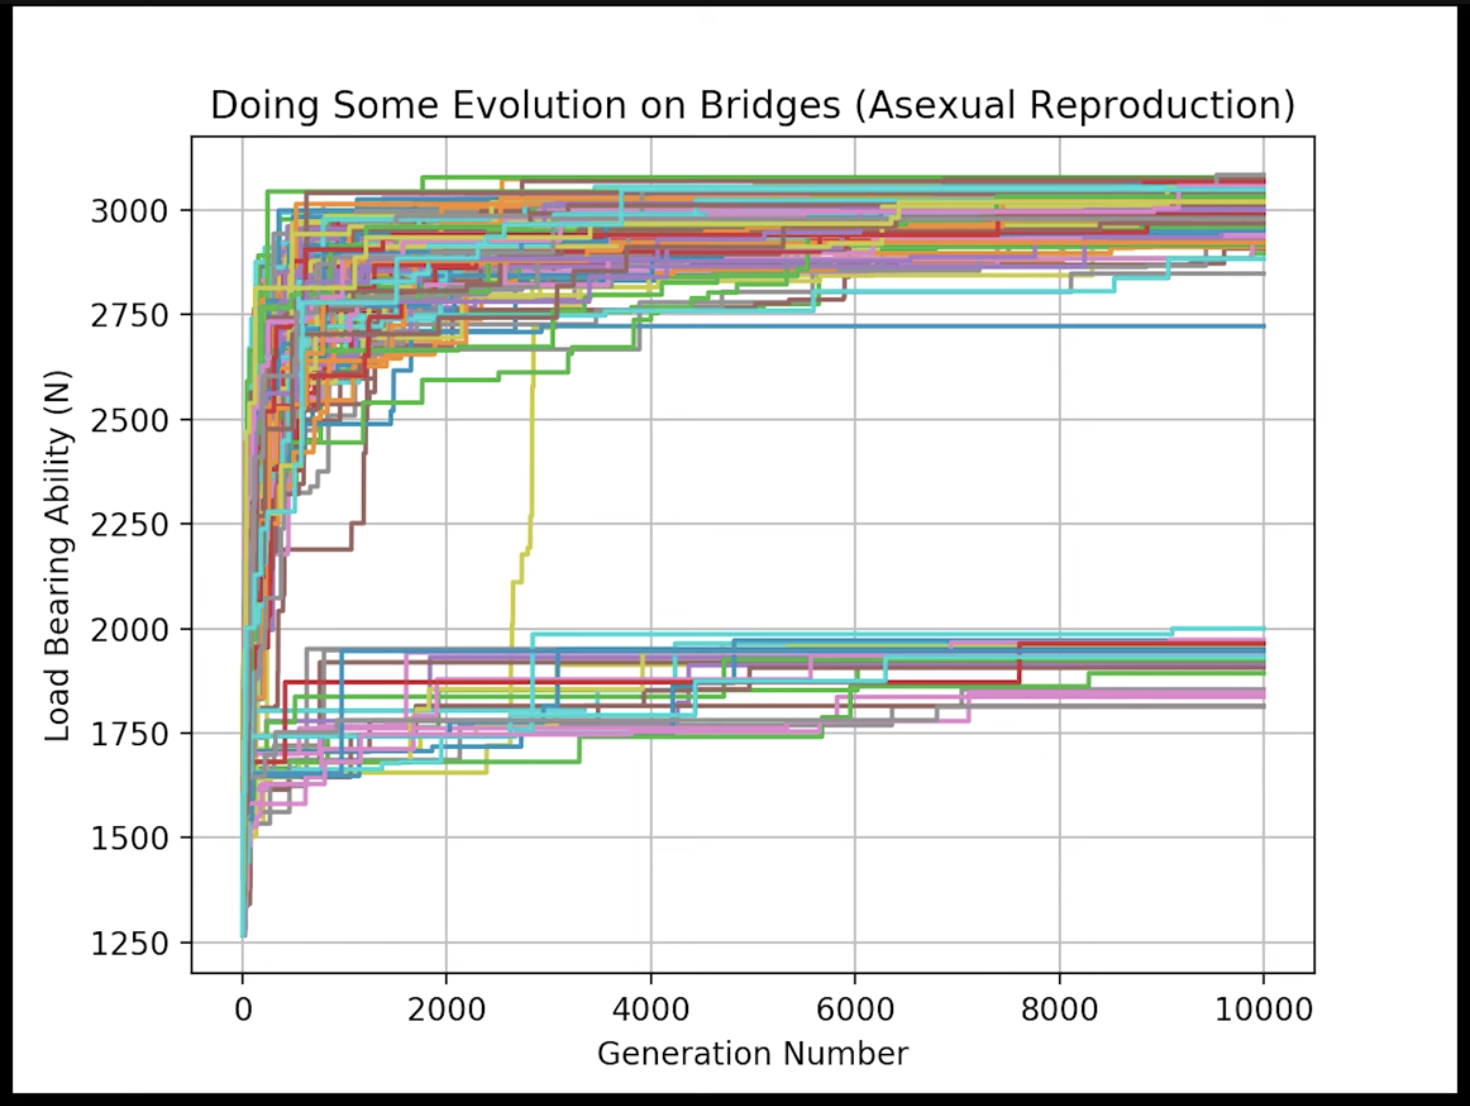
\includegraphics[width=0.7\textwidth]{img/image006.png}
\caption{As I documented this project, I learned the importance of goood data visualization and documentation for a project. In this case, it allowed me to learn that the solution space to the CIV102 bridges gave rise to two \textit{species} that can be seen on this graph.}
\label{}
\end{figure}















\end{document}
